\documentclass[french]{article}
\usepackage[T1]{fontenc}
\usepackage[utf8]{inputenc}
\usepackage{lmodern}
\usepackage[a4paper]{geometry}
\usepackage{babel}
\usepackage{graphicx}

\begin{document}
\title{Nuages de points et modélisation 3D\\
TP 2 : Recalage}
\author{Marius Dufraisse}
\date{}

\maketitle


\paragraph{Question 1.} 
ICP performs well for the bunny only when it is only perturbed, not returned (see Figure \ref{fig:q1-bunny}). For Notre-Dame the results are good too (see Figure \ref{fig:q1-nd12}). The aligned cloud and the reference cloud are not the same as they do not cover the same area. The order used here is important, if the small cloud is used as a reference the ICP will try to align points from the large cloud that don't match points in the small one (see Figure \ref{fig:q1-nd21}). 

\begin{figure}[h]
	\centering
	\begin{minipage}{0.45\linewidth}
		\centering
		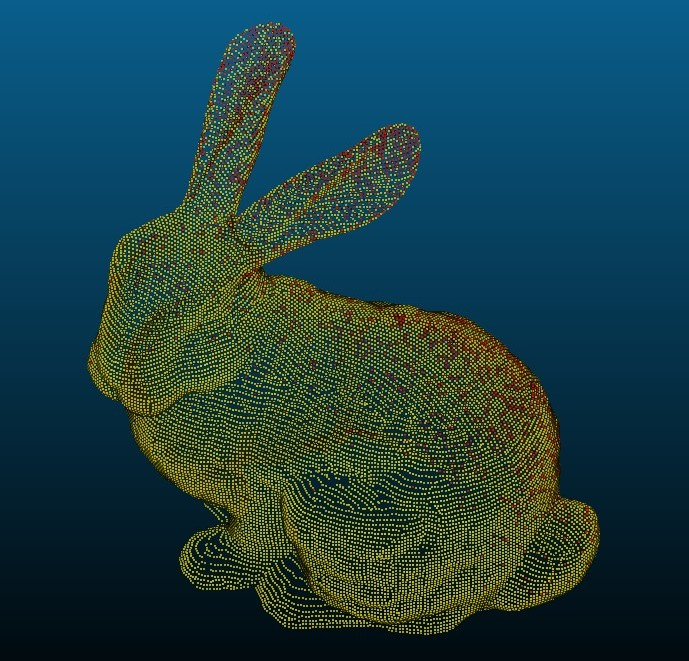
\includegraphics[width=\linewidth]{q1-perturbed.jpg}
	\end{minipage}\hfill
	\begin{minipage}{0.45\linewidth}
		\centering
		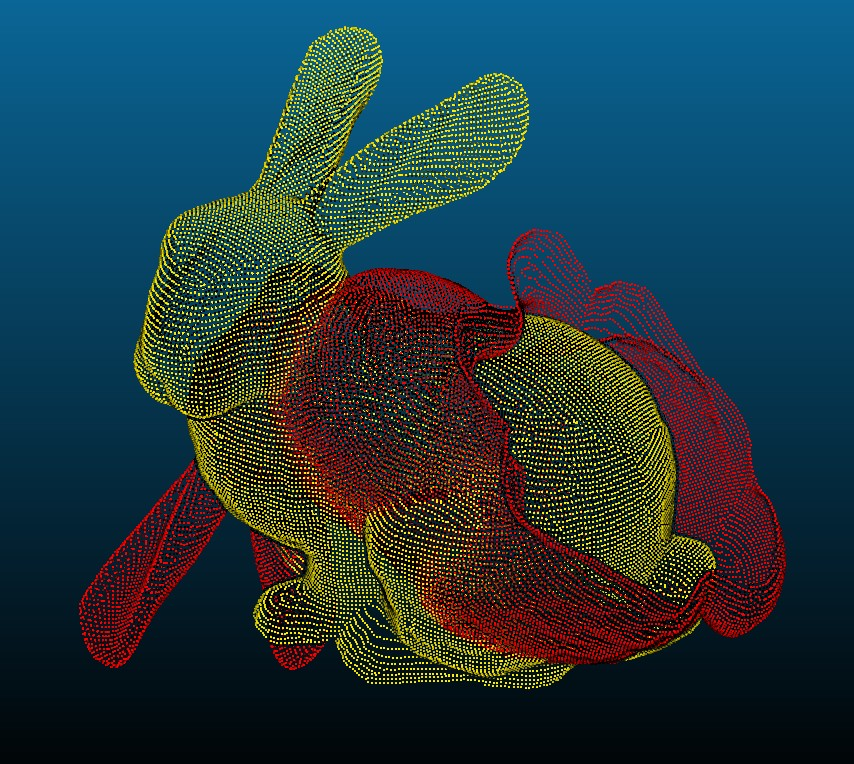
\includegraphics[width=\linewidth]{q1-returned.jpg}
	\end{minipage}
	\caption{Results obtained using CloudCompare implementation of ICP. On the left, the data to align was only slightly perturbed; on the right it was returned.}
	\label{fig:q1-bunny}
\end{figure}

\begin{figure}[h]
	\centering
	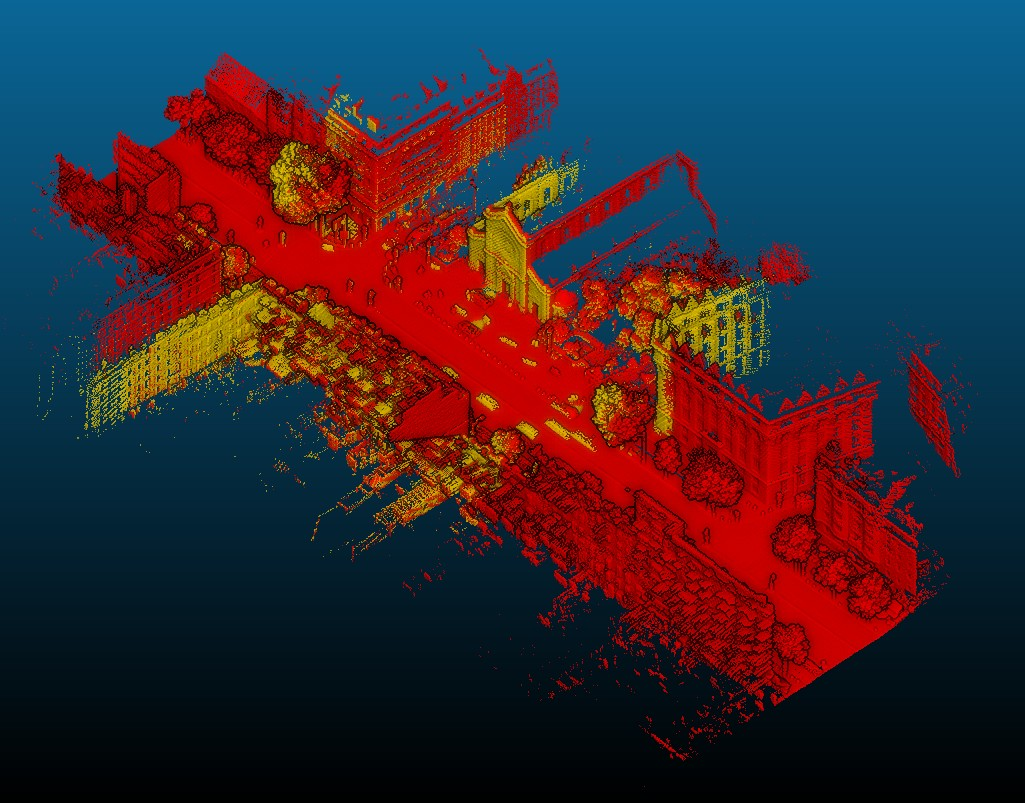
\includegraphics[width=0.6\linewidth]{q1-nd-12.jpg}
	\caption{Results obtained using CloudCompare implementation of ICP on the Notre-Dame point cloud. The larger cloud was used as reference.}
	\label{fig:q1-nd12}
\end{figure}

\begin{figure}[h]
	\centering
	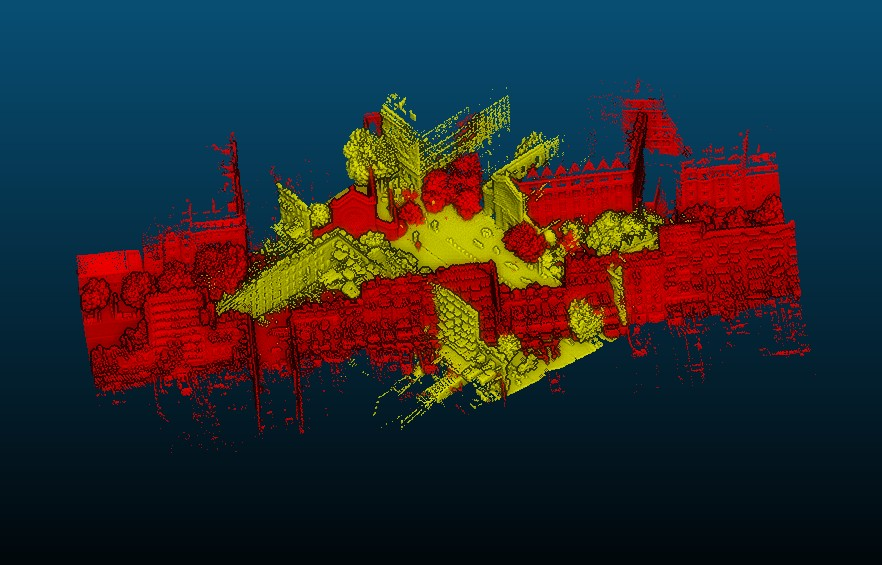
\includegraphics[width=0.6\linewidth]{q1-nd-21.jpg}
	\caption{Results obtained using CloudCompare implementation of ICP on the Notre-Dame point cloud. The smaller cloud was used as reference, as a result the algorithm performed poorly.}
	\label{fig:q1-nd21}
\end{figure}

\paragraph{Question 2.} The RMS between the returned cloud and the reference one was $0.16$. The RMS between the aligned cloud and the reference one was $1.32\times 10^{-8}$. This method worked better than CloudCompare ICP because it uses the fact that the order of the points is the same in both model : this is a strong assumption. For instance it would not work for the Notre Dame clouds as they do not even have the same number of points.

\paragraph{Question 3.}
The graph for RMS convergence during ICP are shown in Figure \ref{fig:q3-2d} and \ref{fig:q3-3d}.

\begin{figure}[h]
	\centering
	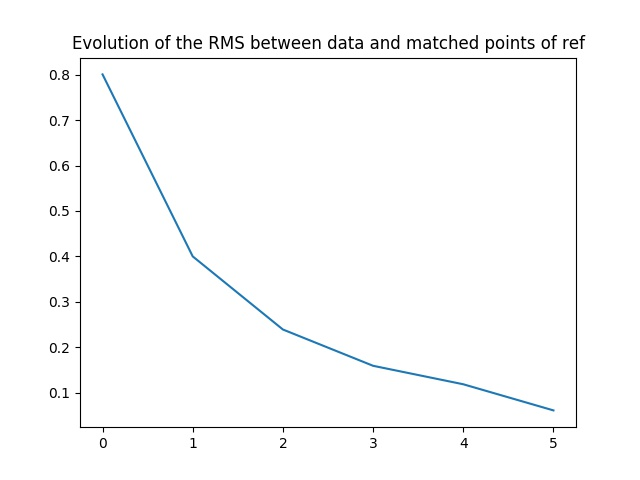
\includegraphics[width=0.5\linewidth]{q3-2D.jpg}
	\caption{Evolution of the RMS for every step of ICP when applied to the 2D example.}
	\label{fig:q3-2d}
\end{figure}

\begin{figure}[h]
	\centering
	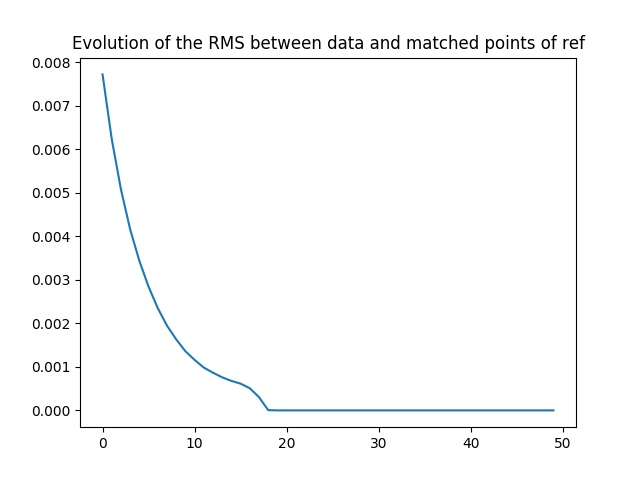
\includegraphics[width=0.5\linewidth]{q3-3D.jpg}
	\caption{Evolution of the RMS for every step of ICP when applied to the perturbed bunny cloud. The RMS goes down to around $1.4\times  10^{-7}$ and then stop decreasing, likely due to rounding errors.}
	\label{fig:q3-3d}
\end{figure}

\paragraph{Question 4.}
The RMS plot for ICP and different number of matched points can be seen in Figure \ref{fig:q4}. Increasing the number of points used at each iteration reduces variance but the final RMS remains fairly high.

\begin{figure}[h]
	\centering
	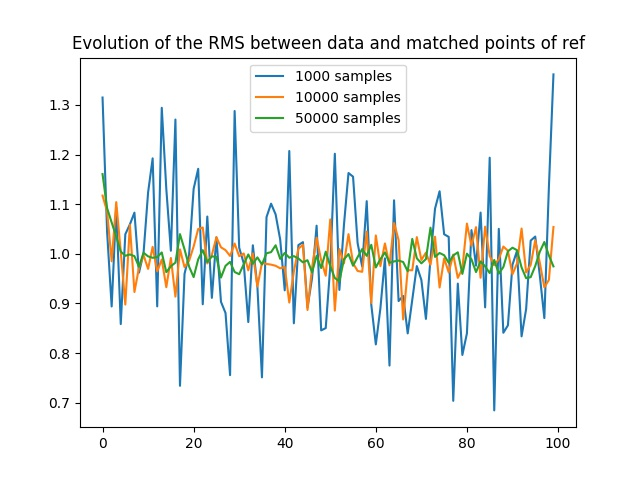
\includegraphics[width=0.6\linewidth]{q4.jpg}
	\caption{Evolution of the RMS during ICP for the Notre Dame cloud.}
	\label{fig:q4}
\end{figure}

\paragraph{Question 5.}
The farthest points do not have a match on the other  cloud, they are on parts of buildings that were not present in the first scan. They are likely to hinder ICP convergence as the algorithm will try find a transformation that maps them to some points in the reference cloud. For the same reason RMS computed on the whole cloud is not really relevant as we expect the distance of some points to the other cloud to remain high.



\end{document}
